\title{Exploiting Heap Overflows on ARM}
\author{
    Author: Yusef Karim \\
    Instructor: Jacques Béland \\
    Department of Computing \& Information Systems \\
}
\date{\today}

\documentclass[12pt]{article}
\usepackage[utf8]{inputenc}
\usepackage[english]{babel}
\usepackage[a4paper,margin=1in,footskip=0.25in]{geometry}
\usepackage[colorlinks=true]{hyperref}
\usepackage{graphicx}
\usepackage{float}

\begin{document}
\maketitle
\tableofcontents

\section{Purpose}
This is a mini lab that will explore heap based exploits. This is covered in chapter 5 of the course text but several external resources were used instead.

\section{What is the Heap?}
The heap is a program segment that memory can be allocated to just like the stack, although the stack and heap both allow memory allocation, heap memory is very different. Memory allocation using the heap is usually not done during compilation time but during run time and can be of arbitrary size and order. Memory allocated on the heap is globally accessible, compared to the stack which gets allocated during a function call and destroyed before the function returns.\newline

In a C program the functions \textit{malloc()} and \textit{free()} are used to allocate and free memory respectively. Malloc uses the system calls \textit{brk} or \textit{sbrk} to grow the heap [1], this memory can be accessed using pointers to the memory addresses within the heap.\newline

A common issue with heap allocation is memory fragmentation. For example if a programmer were to allocate three variables on the heap using \textit{malloc()} let's say a, b, c, then free the variable b before a and c, there would be a hole between these two variables. This memory can sometimes be retrieved by \textit{malloc()} when it tries to organize the heap but if not, memory fragmentation will occur. This has caused several different implementations of \textit{malloc()} to be created such as dlmalloc, jemalloc, and ptmalloc which all allocate and organize memory differently.\newline

One last point is where the heap allocates memory. We know in general the stack starts at a very high memory address then grows towards lower memory addresses, the heap does the exact opposite. To explore this let's use gdb to print the memory layout of a program. This program is called hello.c is located in the lab4\_code directory.

\begin{figure}[H]
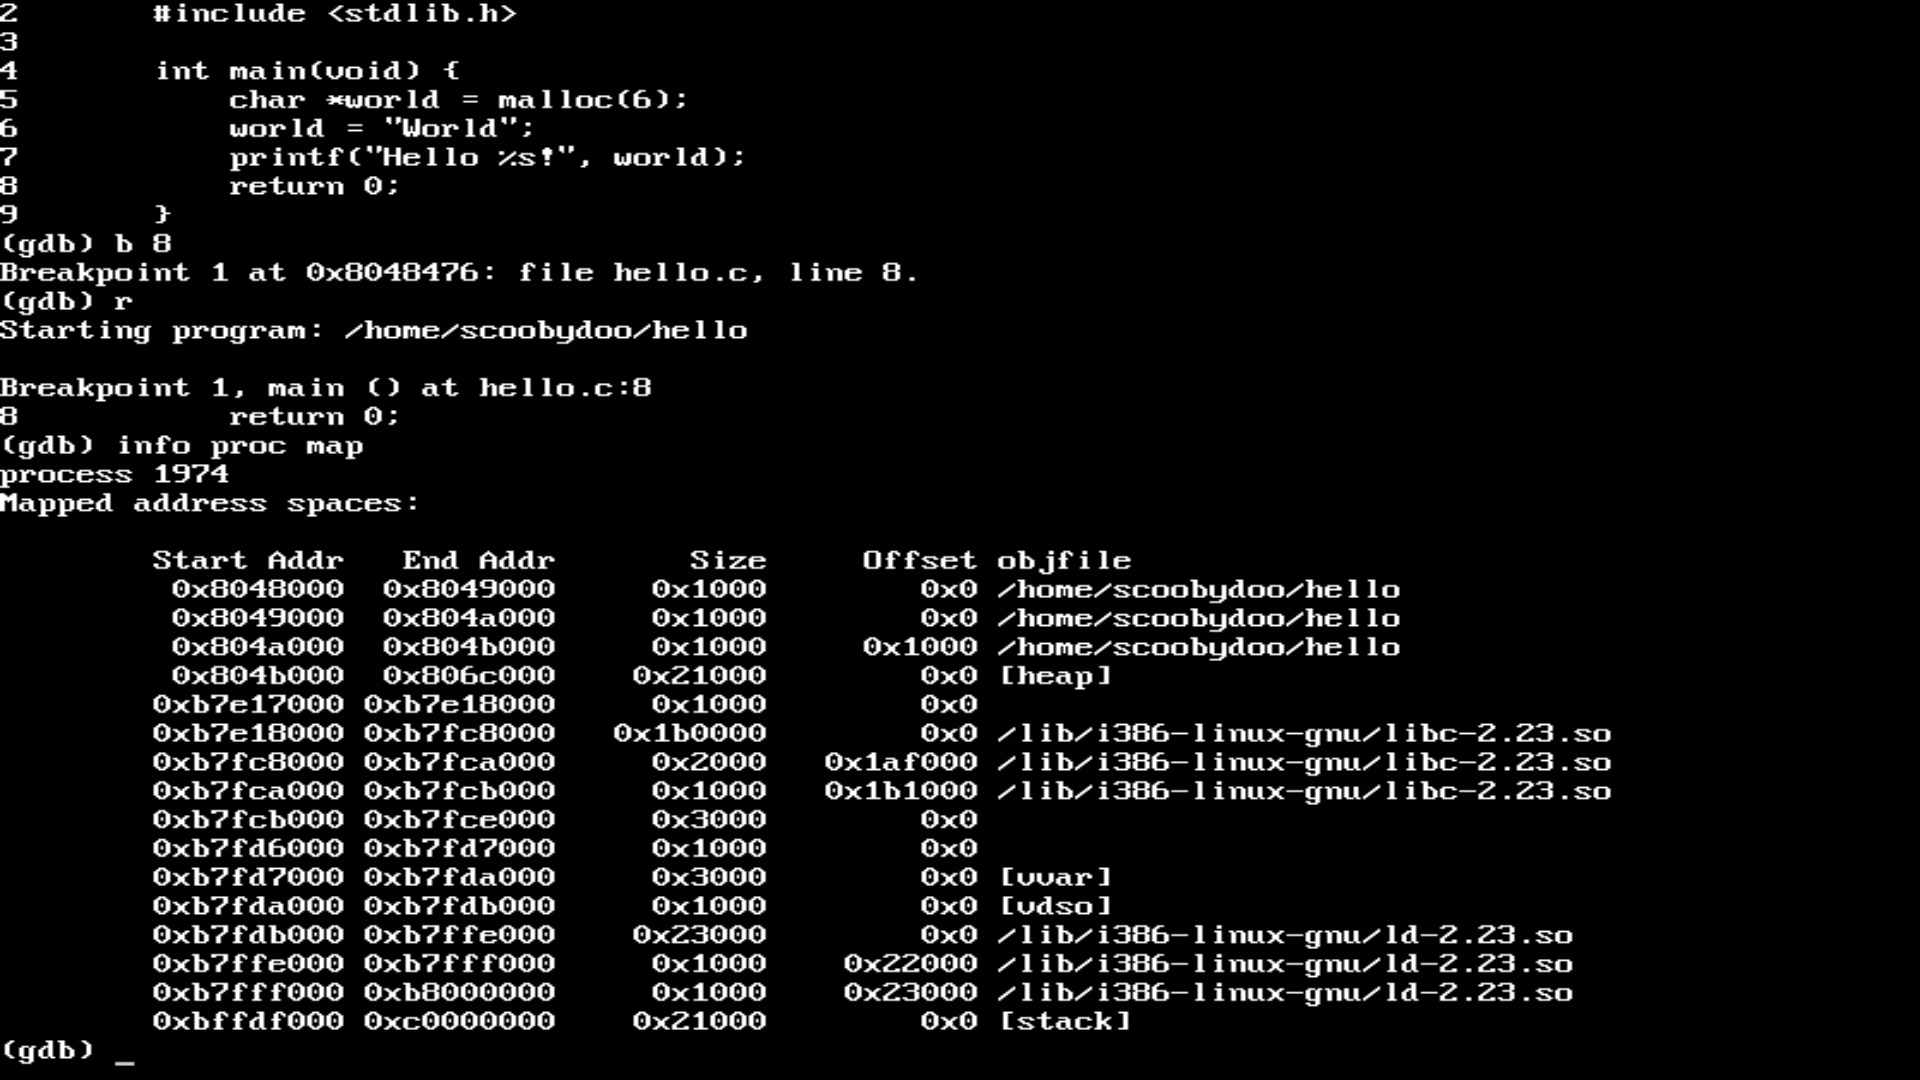
\includegraphics[width=15cm, height=8cm]{heap_gdb.png}
  \caption{Exploring memory layout of hello.c}
\end{figure}

We can see that the variable \textit{world} has been allocated in the heap using malloc, then using the gdb command \textit{info proc map} we see that the heap does indeed start at a much lower address than the stack that has been created.

\section{Controlling program flow after exploiting the Heap}
In our previous labs we have been dealing solely with stack-based overflows so before we jump into heap overflows let's think about how we can control the flow of execution if we actually are able to exploit the heap.\newline

When exploiting the stack, we always aimed to overwrite the Instruction Pointer\textbackslash Program Counter since this register is stored on the stack before a function call. This allowed us to change the return address of whatever function was being called to something of our liking. This is not going to happen when exploiting the heap, at least not directly (foreshadowing). Through my readings, it seems like a very common thing to try and overwrite with heap-overflows is the Global Offset Table (GOT). The GOT contains the address of linked functions (functions in libc for example) which the program can look up then call. If we are able to overwrite an address entry in the GOT with the address of our shellcode, then when the program executes that entry in the GOT it will call our shellcode instead of the intended function. Great, but before we start let's learn about how the GOT gets those addresses in its table and how our program knows what to look for in the GOT.\newline

To explore this I have decided to use a vulnerable program called heap1.c from exploit-exercises.com [2]. This is mainly due to the mass amounts of documentation on this program, I used a youtube video by LiveOverflow [3] to learn about the exploit. Also, since there is so much documentation on this for x86 I have decided to focus primarily on ARM. That being said, let's get back to learning about the Global Offset Table before we actually exploit heap1.c.\newline

To begin, let's compile heap1.c and keep in mind that when we compile a program using GCC it creates an executable in the Executable and Linking Format (ELF).

\begin{verbatim}
  gcc heap1.c -fno-stack-protector -o heap1
\end{verbatim}

We can then use the GNU program \textit{readelf} to list out the sections of our ELF executable.

\begin{figure}[H]
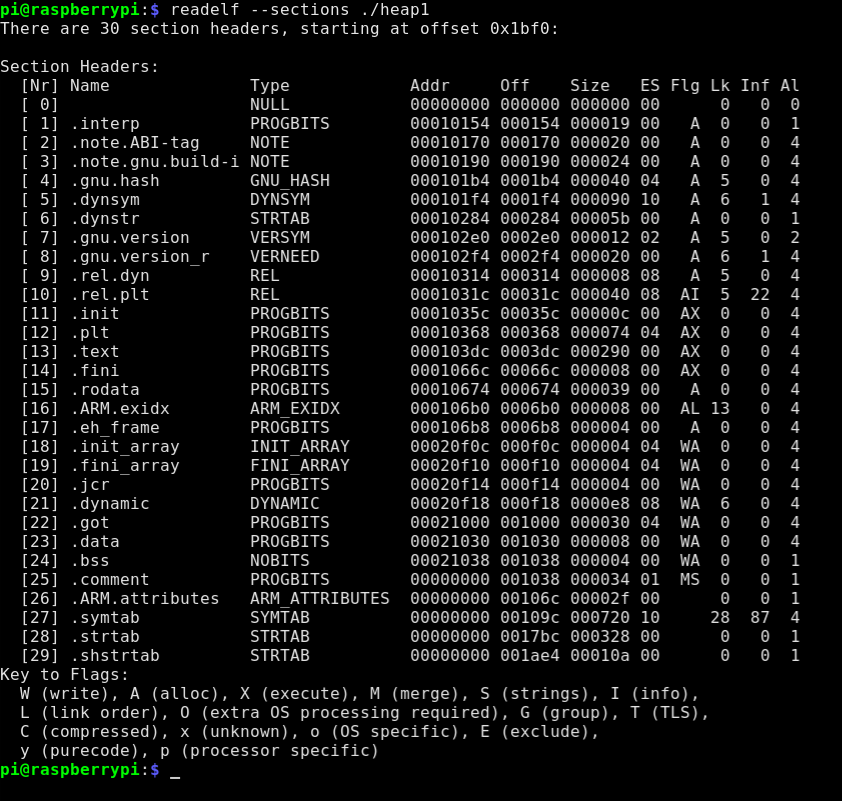
\includegraphics[width=15cm, height=10cm]{sections.png}
  \caption{Section headers in heap1.c}
\end{figure}

There are two important things we need to pay attention too, first is the \textbf{.got} section which starts at 0x00021000, second the \textbf{.plt} section which stands for Procedure Lookup Table (PLT) which starts at 0x00010368, we will see why this table is relevant soon. Next, we can use \textit{readelf} again to see the offsets from the start of the GOT to all the relevant functions our program needs.

\begin{figure}[H]
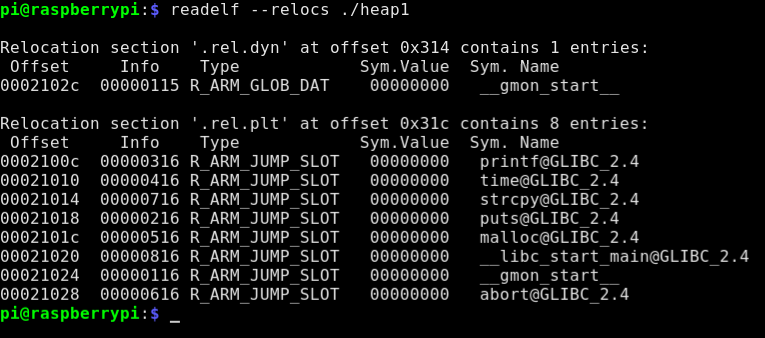
\includegraphics[width=15cm, height=7cm]{relocs.png}
  \caption{Relocation sections in heap1.c}
\end{figure}

This doesn't tell us much right away other than the fact that there is libc functions located within the GOT at specific offsets. Let's jump into GDB now so we can understand what the heck is actually going on.

\begin{figure}[H]
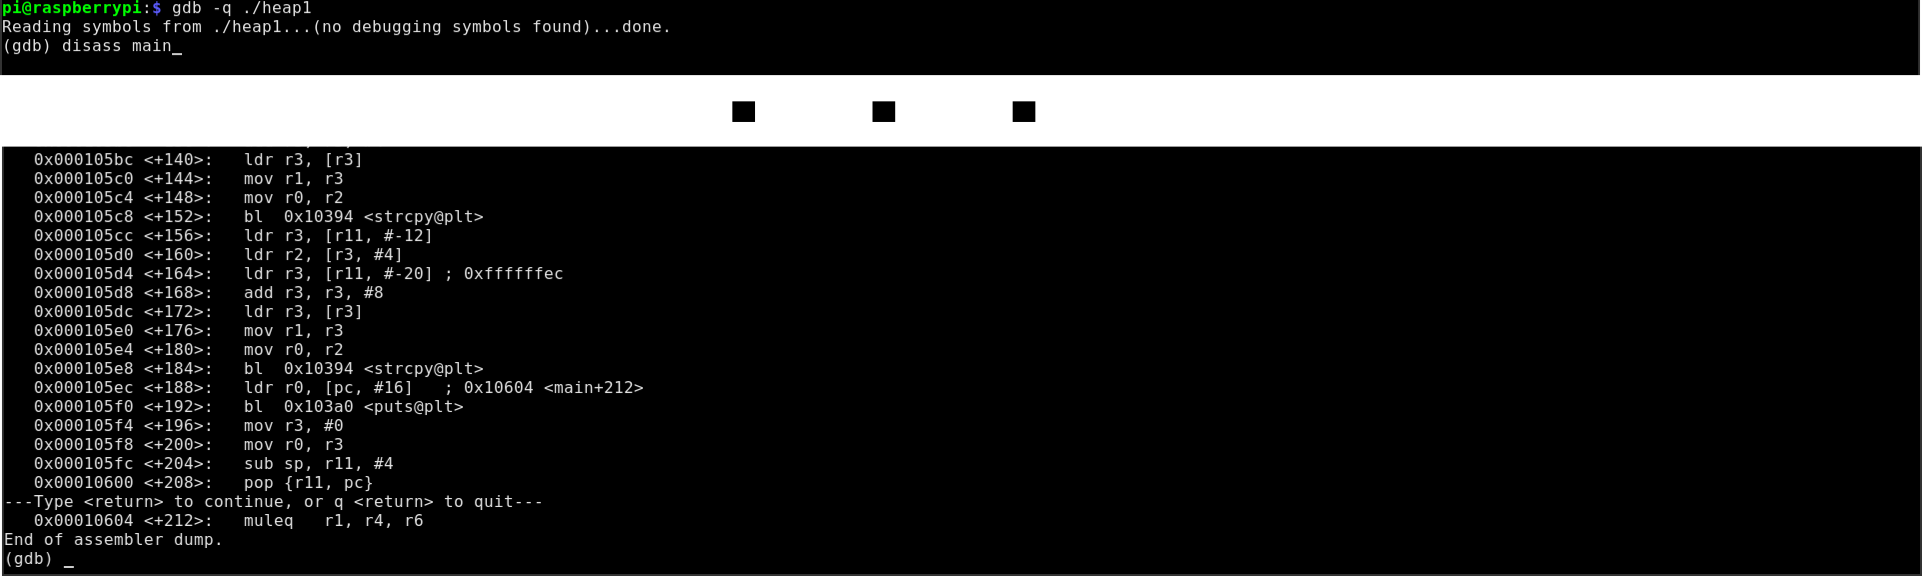
\includegraphics[width=15cm, height=10cm]{gdb1.png}
  \caption{Bottom half of disassembled main in heap1.c}
\end{figure}

If we look at main+192 we can see a call to the \textit{puts} function, but the word next to it is plt, let's disassemble \textit{puts} and learn what the Procedure Lookup Table actually does.

\begin{figure}[H]
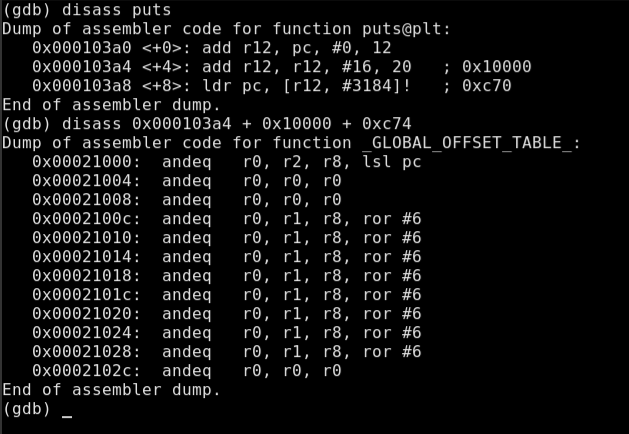
\includegraphics[width=15cm, height=7cm]{gdb2.png}
  \caption{Disassembly of puts in heap1.c}
\end{figure}

The \textit{puts} disassembly output actually takes us to the .plt section of our code, and this section uses a set of instructions to calculate something and then loads that value into the Program Counter (PC). The value that is being calculated is actually the offset to the address of the actual linked puts function in the Global Offset Table (GOT). If we were to calculate the value being loaded into PC (0x000103a4 + 0x10000 + 0xc74) we would see that it turns out to be 0x21018 which if we look at the relocation offsets in Figure 3 above, we will see it points directly at the \textit{puts} function in the GOT. Cool, so the PLT contains instructions to calculate the address in the GOT then the GOT table calls \textit{puts}, but wait when we look at the GOT in GDB it looks like a bunch of fooey. This is because the GOT initially contains instructions to call the Dynamic Linker (ld) which is linked to our program. The Dynamic Linker will then go find the function address from libc and store it in the GOT, this is to avoid extra code and large binaries, the Dynamic Linker will just find the function the program needs when it needs it then store it in the GOT so anytime the program needs that function again it can just look directly at the GOT [4][5].\newline

What would happen if we were to overwrite the address of \textit{puts} in the GOT before the program calls \textit{puts}? Let's find out.

\section{Exploiting the Heap}
If we take a look at the \textit{heap1.c} source code there are 3 lines that tell us almost all we need right away.
\begin{verbatim}
  strcpy(i1->name, argv[1]);
  strcpy(i2->name, argv[2]);

  printf("and that's a wrap folks!\n");
\end{verbatim}
From the disassembly in Figure 4 we already know that the code uses malloc to allocate strings, we also see the last function call in the program is actually \textit{puts} not \textit{printf} this is probably an optimization made by the compiler. From the 3 lines above we see this program uses the vulnerable \textit{strcpy} function to copy the first two command line arguments passed into the program. How can we take advantage of this?\newline

Since we know how the GOT table works, we can try to pass a large buffer to the program as the first argument, since the heap allocations are likely contiguous we will write past the i1->name buffer and eventually start overwriting the address of the i2->name. That means we could theoretically overwrite the address i2->name points to, then use the second \textit{strcpy} function to write the value we want to that overwritten address. Let's try it!\newline

Let's be a little methodical about it though. If we look at the man pages for the \textit{malloc} function we see it returns a pointer to the allocated memory, so let's get the actual memory address of the i2->name string by setting a breakpoint after the third \textit{malloc} call, \textit{malloc} will store the return address of the allocated memory in R0 and i2->name will be 4 bytes beyond this since it is after the integer in the internet structure.

\begin{figure}[H]
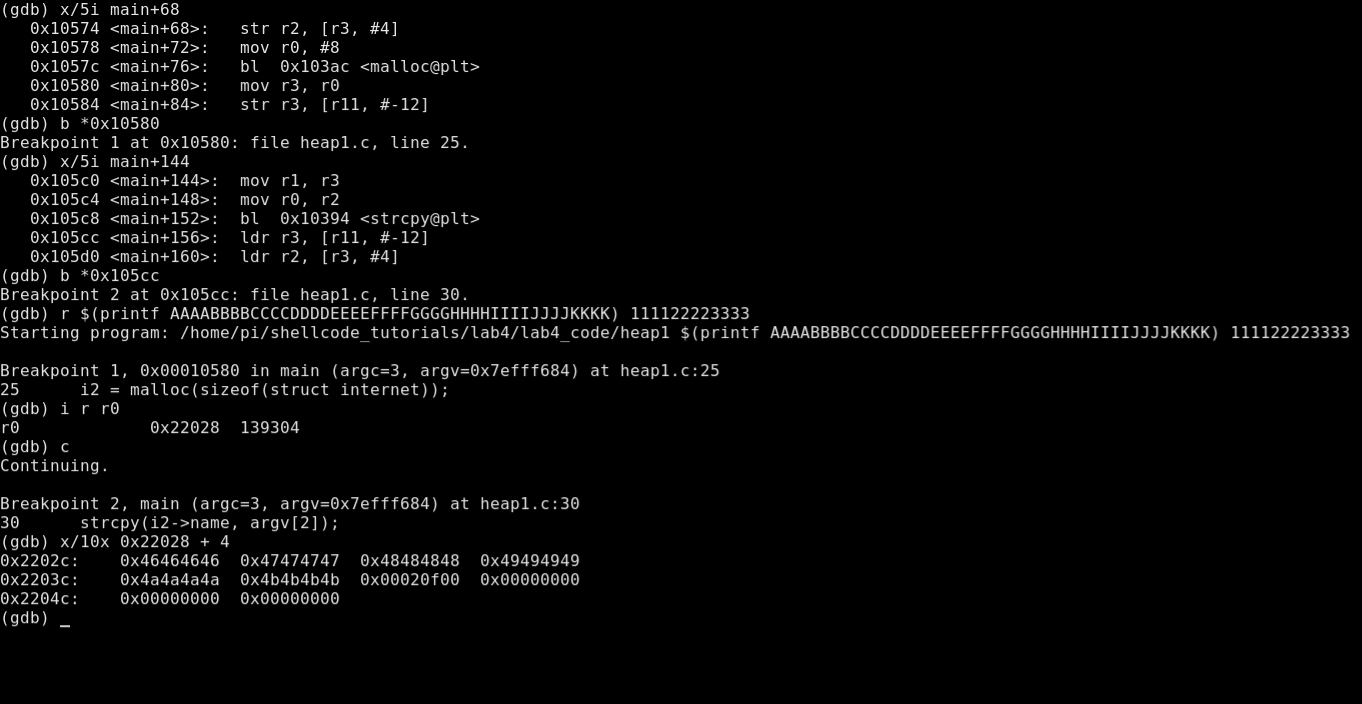
\includegraphics[width=15cm, height=7cm]{gdb3.png}
  \caption{Finding offset to overflow i2->name}
\end{figure}

In the Figure above, we set a breakpoint right after the internet structure gets allocated, then another breakpoint on the \textit{strcpy} that copies the first command line argument into the i1->name buffer. We then run the program with a large buffer for both the first and second command line argument. After running we hit the first breakpoint and see that \textit{malloc} returned the address 0x22028, this means the address 0x2202c will be the address of the i2->name string. We continue to the next breakpoint and print the values starting at the i2->name string. We can now clearly see the heap buffer started to overflow after 20 bytes (AAAABBBBCCCCDDDDEEEE). Great, almost there, we can put the address of the GOT value for the \textit{puts} function which we found in Figure 3 (0x21018) after our 20 byte offset. This will overflow the value i2->name points too then the \textbf{second} \textit{strcpy} will copy the value we pass as the second argument into the address i2->name points too. Let's give the address of the \textit{winner} function as the second argument.

\begin{figure}[H]
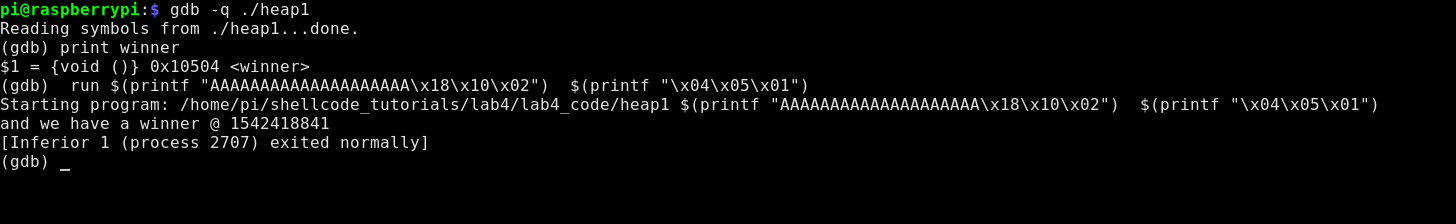
\includegraphics[width=15cm, height=3.5cm]{gdb4.png}
  \caption{Overwriting the GOT with the \textit{winner} function}
\end{figure}

It worked! We used the first \textit{strcpy} to overflow the address i2->name points too with the GOT value for \textit{puts}, the second \textit{strcpy} function then wrote the address of the \textit{winner} function into the GOT, the call to \textit{puts} then called the \textit{winner} function instead of \textit{puts}. Let's try this again but with an environment variable containing our shellcode!
\begin{verbatim}
gcc heap1.c -fno-stack-protector -z execstack -o heap1
as good_shell.s -o good_shell.o
ld good_shell.o -N -o good_shell
objcopy -O binary good_shell good_shell.bin
export XSHELLY=$(cat good_shell.bin)           # CHECK YOUR ALIGNMENT!!!!!
\end{verbatim}

\begin{figure}[H]
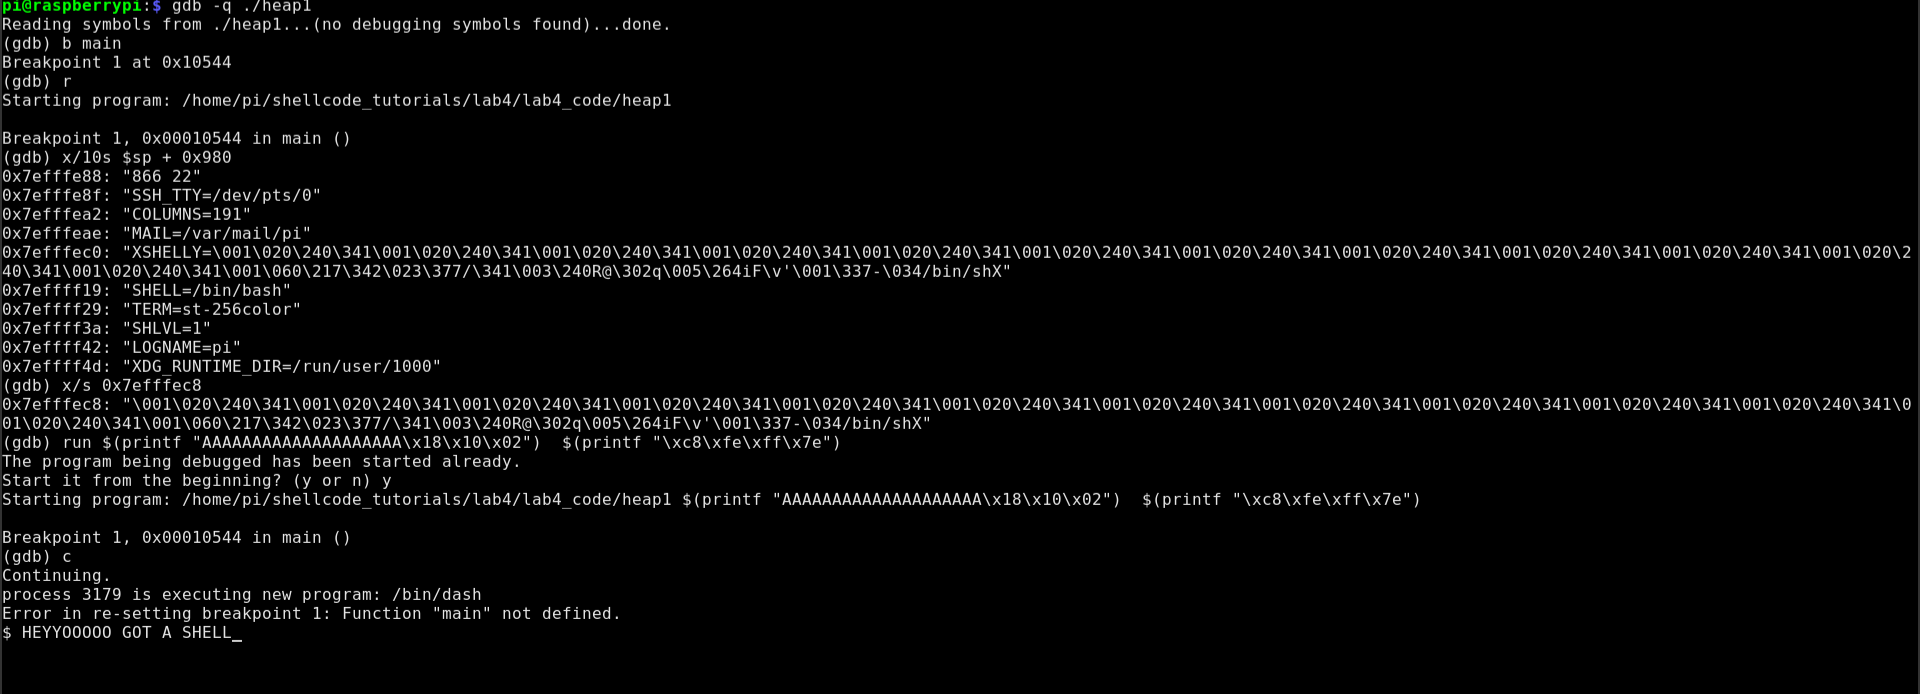
\includegraphics[width=15cm, height=7.5cm]{gdb5.png}
  \caption{Overwriting the GOT with environment variable storing shellcode}
\end{figure}

Awesome! We were able to use the address of our shellcode environment variable as the second argument which \textit{puts} then called for us since we overwrote the GOT value for it.

\section{Conclusion}
Although the example we used was quite exaggerated (doubt this would ever happen in production code) we learned a ton of valuable information about heap memory, the Global Offset Table and the Procedure Lookup Table. We also got to spawn another shell, yahoo!

\section{References}

\begin{enumerate}
  \item\textbf{Heap Memory in C Programming}
    \newline\url{https://stackoverflow.com/questions/10200628/heap-memory-in-c-programming}
  \item\textbf{Heap1.c exploit-exercises.com}
    \newline\url{https://web.archive.org/web/20140405141230/http://exploit-exercises.com/protostar/heap1}
  \item\textbf{LiveOverflow: How to exploit a Heap Overflow}
    \newline\url{https://www.youtube.com/watch?v=TfJrU95q1J4}
  \item\textbf{Global Offset Tables}
    \newline\url{http://bottomupcs.sourceforge.net/csbu/x3824.htm}
  \item\textbf{The Procedure Lookup Table}
    \newline\url{http://bottomupcs.sourceforge.net/csbu/x3882.htm}
\end{enumerate}


\end{document}
